\documentclass[runningheads]{llncs}
%
\usepackage{graphicx}
% Used for displaying a sample figure. If possible, figure files should
% be included in EPS format.
\usepackage{tikz}
\usetikzlibrary{arrows}
\usepackage{verbatim}
%\usepackage{amsmath}
%\usepackage{amssymb}
%\usepackage{graphicx}
%\usepackage[all]{xy}
\usepackage{array}
\usepackage{enumitem}
%\usepackage{cite}
\usepackage[numbers,sectionbib]{natbib}
% If you use the hyperref package, please uncomment the following line
% to display URLs in blue roman font according to Springer's eBook style:
% \renewcommand\UrlFont{\color{blue}\rmfamily}
\usepackage[breaklinks=true]{hyperref}
\usepackage{breakcites}
\renewcommand\UrlFont{\color{blue}\rmfamily}

\usepackage{xcolor}
\usepackage{listings}
\definecolor{dkgreen}{RGB}{0,70,70}
\definecolor{ltblue}{RGB}{0,130,130}
\definecolor{dkviolet}{RGB}{140,0,210}
\definecolor{dkblue}{RGB}{0,0,140}
\definecolor{dkred}{RGB}{140,20,0}
\definecolor{dkorange}{RGB}{130,70,0}

% lstlisting coq style (inspired from a file of Assia Mahboubi)
\lstdefinelanguage{Coq}{ 
    % Anything betweeen $ becomes LaTeX math mode
    mathescape=true,
    % Comments may or not include Latex commands
    texcl=false, 
    % Vernacular commands
    morekeywords=[1]{Section, Module, End, Require, Import, Export,
        Variable, Variables, Parameter, Parameters, Axiom, Hypothesis,
        Hypotheses, Notation, Local, Tactic, Reserved, Scope, Open, Close,
        Bind, Delimit, Definition, Let, Ltac, Fixpoint, CoFixpoint, Add,
        Morphism, Relation, Implicit, Arguments, Unset, Contextual,
        Strict, Prenex, Implicits, Inductive, CoInductive, Record,
        Structure, Canonical, Coercion, Context, Class, Global, Instance,
        Program, Infix, Theorem, Lemma, Corollary, Proposition, Fact,
        Remark, Example, Proof, Goal, Save, Qed, Defined, Hint, Resolve,
        Rewrite, View, Search, Show, Print, Printing, All, Eval, Check,
        Projections, inside, outside, Def},
    % Gallina
    morekeywords=[2]{forall, exists, exists2, fun, fix, cofix, struct,
        match, with, end, as, in, return, let, if, is, then, else, for, of,
        nosimpl, when},
    % Sorts
    morekeywords=[3]{Type, Prop, Set, true, false, option},
    % Various tactics, some are std Coq subsumed by ssr, for the manual purpose
    morekeywords=[4]{pose, set, move, case, elim, apply, clear, hnf,
        intro, intros, generalize, dependent, constructor, subst, rename, pattern, after, destruct, induction, using, refine, inversion, injection, rewrite, congr, unlock, compute, ring, field, fourier, replace, fold, unfold,
        change, cutrewrite, simpl, have, suff, wlog, suffices, without,
        loss, nat_norm, assert, cut, trivial, revert, bool_congr, nat_congr,
        symmetry, transitivity, auto, split, left, right, autorewrite},
    % Terminators
    morekeywords=[5]{by, done, exact, reflexivity, tauto, romega, omega,
        assumption, solve, contradiction, discriminate},
    % Control
    morekeywords=[6]{do, last, first, try, idtac, repeat},
    % Comments delimiters, we do turn this off for the manual
    morecomment=[s]{(*}{*)},
    % Spaces are not displayed as a special character
    showstringspaces=false,
    % String delimiters
    morestring=[b]",
    morestring=[d],
    % Size of tabulations
    tabsize=3,
    % Enables ASCII chars 128 to 255
    extendedchars=false,
    % Case sensitivity
    sensitive=true,
    % Automatic breaking of long lines
    breaklines=false,
    % Default style fors listings
    basicstyle=\small,
    % Position of captions is bottom
    captionpos=b,
    % flexible columns
    columns=[l]flexible,
    % Style for (listings') identifiers
    identifierstyle={\ttfamily\color{black}},
    % Style for declaration keywords
    keywordstyle=[1]{\ttfamily\color{dkblue}},
    % Style for gallina keywords
    keywordstyle=[2]{\ttfamily\color{dkgreen}},
    % Style for sorts keywords
    keywordstyle=[3]{\ttfamily\color{ltblue}},
    % Style for tactics keywords
    keywordstyle=[4]{\ttfamily\color{dkorange}},
    % Style for terminators keywords
    keywordstyle=[5]{\ttfamily\color{dkred}},
    %Style for iterators
    keywordstyle=[6]{\ttfamily\color{dkviolet}},
    % Style for strings
    stringstyle=\ttfamily,
    % Style for comments
    commentstyle={\ttfamily\color{dkgreen}},
    %moredelim=**[is][\ttfamily\color{red}]{/&}{&/},
    literate=
    {forall}{{$\forall\;$}}1
    {exists}{{$\exists\;$}}1
    {\\subsetOf}{{$\subseteq\;$}}1
    {<-}{{$\leftarrow\;$}}1
    {=>}{{$\Rightarrow\;$}}1
    {==}{{\code{==}\;}}1
    {==>}{{\code{==>}\;}}1
    %    {:>}{{\code{:>}\;}}1
    {->}{{$\rightarrow\;$}}1
    {<->}{{$\leftrightarrow\;$}}1
    {<==}{{$\leq\;$}}1
    {\#}{{$^\star$}}1 
    {\\o}{{$\circ\;$}}1 
    {\@}{{$\cdot$}}1 
    {\/\\}{{$\wedge\;$}}1
    {\\\/}{{$\vee\;$}}1
    %{++}{{\code{++}}}1
    {~}{{$\neg$}}1
    {<>}{{$\neq$ }}1
    {\@\@}{{$@$}}1
    {\\mapsto}{{$\mapsto\;$}}1
    {\\hline}{{\rule{\linewidth}{0.5pt}}}1
    %
}[keywords,comments,strings]

\begin{document}
%
\title{Verifying TPM DevID Provisioning\thanks{This work is funded in part
    Honeywell FMT Purchase Order
    \#N000422909. The views and conclusions contained in this document
    are those of the authors and should not be interpreted as
    representing the official policies, either expressed or implied,
    of the U.S. Government.}}
%
%\titlerunning{Abbreviated paper title}
% If the paper title is too long for the running head, you can set
% an abbreviated paper title here
%
\author{Sarah Johnson \and
Perry Alexander}
%
\authorrunning{S. Johnson and P. Alexander.}
% First names are abbreviated in the running head.
% If there are more than two authors, 'et al.' is used.
%
\institute{Institute for Information Sciences \\ The
  University of Kansas \\ Lawrence, KS 66045 \\
  \email{\{sarahjohnson,palexand\}@ku.edu}}
%
\maketitle              % typeset the header of the contribution
%
\begin{abstract}
  Provisioning TPM-based secure device identifiers must be verified
  to ensure they are strongly bound to their devices.
  Lack of such assurance jeopardizes high-integrity decisions and
  reporting that rely upon associating data with devices.  We develop
  models of two TCG provisioning protocols and verify they provide
  assurances necessary to produce a strong cryptographic binding
  of TPM key to device.  As a result we can be assured that initial
  and local device identifiers are strongly bound to their associated
  devices.

  \keywords{Secure Device Identifiers \and TPM \and Verification.}
\end{abstract}
%
%
%
\section{Introduction}

Deployment of trusted systems requires strong
identification~\citep{Martin:08:The-ten-page-in} ensuring a remote
device is unambiguously associated with an identity. Strong identity
has two properties: (i) generated and bound to the device using good
credentials (integrity); and (ii) stored in a way that prevents use by
other devices (confidentiality).  Without strong identification a
malicious source can produce and use an invalid identity or steal and
use the identity of good entity.

One method for implementing strong identity is a \emph{secure device
  identifier (DevID)}~\citep{DevIDSpec-IEEE} realized using a Trusted
Platform Module (TPM) to generate and protect DevID instances. 
The Trusted Computing Group DevID Specification~\citep{DevIDSpec-TCG}
describes protocols for assuring DevID integrity and
confidentiality. These protocols are performed by a trusted Certificate 
Authority (CA) communicating with a certificate-requesting device.
The protocols result in the formation of a cryptographic evidentiary chain 
linking a DevID to its TPM-containing device and produce a certificate 
assuring integrity.  Furhtermore, the TPM provides an attribute that when set during 
key creation prevents duplication or sharing of a key.
The protocols verify this attribute is set for a DevID assuring confidentiality.
%% First,
%% the Trusted Computing Group DevID Specification~\citep{DevIDSpec-TCG}
%% describes protocols for assuring DevID integrity and residency. These
%% protocols are performed by a trusted Certificate Authority (CA)
%% communicating with a certificate-requesting device.  They evaluate a
%% cryptographic evidentiary chain linking a DevID to its TPM-containing
%% device and produce a certificate assuring integrity.  Second, the TPM
%% provides an attribute that when set during key creation
%% prevents duplication or sharing of a key. Setting this attribute for
%% a DevID key ensures its confidentiality.

Our work focuses on correctness of two certification protocols:
(i) OEM Creation of an IAK Certificate based on an EK Certificate; and
(ii) Owner Creation of an LAK Certificate based on an IAK
Certificate. These DevID establishment protocols and their resulting
certificates are essential for our work in remote
attestation~\citep{Coker::Principles-of-R,petz2022innovations} where
device appraisal requires strong identification of an attestation
source. Specifically, ensuring the signing key for an attestation
result is bound to the attestation manager responsible for that
attestation.  Contributions of this research include: (i) design and
implementation of an abstract formal model of TPM command execution;
(ii) an in-depth analysis of the TCG-provided IAK and LAK
certification protocols, and (iii) a recommendation for clarifying the
IAK provisioning procedure.

\section{DevIDs and TPMs}
The \emph{Trusted Platform Module (TPM)} is a microcontroller that complies
with the ISO/IEC 11889:2015 international standard.  The TPM was
designed by the Trusted Computing Group (TCG) to act as a hardware
root-of-trust for PC system security.  TPMs are increasingly common
making them a strong choice for building DevIDs.

%%\subsection{TPM Keys and DevID Certificates}
In the context of this work, a \emph{TPM key} is an asymmetric key created
and used by a TPM in a way that is consistent with its specified attributes.
TPM key attributes are permanent, set at creation-time, and restrict how the key may
be used. Attributes include \verb|FixedTPM| to control duplication,
\verb|Sign| and \verb|Decrypt| to restrict the key usage, and
\verb|Restricted| to limit operations to TPM-generated data only.  A
restricted decryption key is called a \emph{storage key} while a
restricted signing key is call an \emph{attestation key (AK)}.  
The AK is so named for its unique ability to prove that a data
object is contained in the same TPM as the key itself.

%% Primary TPM keys are maintained internally by the TPM as roots for
%% chaining key ownership. They are shielded and not available outside
%% the TPM.  Ordinary TPM keys are wrapped by a parent TPM key and can be
%% stored outside the TPM.  The wrapping operation encrypts the ordinary
%% TPM key's private key with a parent public key and includes a PCR
%% composite. The public key remains clear and can be used for encryption
%% and signature checking.  However, decryption and signing are possible
%% only if both key and its parent are installed in the TPM.  When the
%% key is installed the parent key must be installed to decrypt its
%% private key.  Wrapping creates an ownership chain from ordinary keys
%% to a primary key, thus binding keys in the chain to the TPM.



% key may only sign a PCR digest produced by the TPM during attestation
% and to prove that a new key is loaded on the same TPM as itself during
% certification.  A valid signature proves that quoted PCR values or new
% key are from the same TPM as the original key.  If the signing key is
% bound to the a TPM, then the PCR values or new key are also bound to
% the same TPM.

% A restricted decryption key is called a storage key. Only storage keys
% can be used as parents to create or load child objects or to activate
% credentials~\citep{PracticalGuide}. The EK is initialized by the TPM
% manufacturer and stored in a shielded location on the TPM. The
% corresponding EK certificate is the root certificate for chains of
% IAKs and LAKs and thus plays a significant role in the creation of
% DevID certificates.

A \emph{secure device identifier (DevID)} is a TPM key with
\verb|FixedTPM| and \verb|Sign| set, cryptographically bound to a
device by a \emph{DevID certificate}.  Thus, a DevID is a signing key
that cannot be duplicated or shared outside the TPM.  The
\verb|FixedTPM| attribute is essential as it guarantees the
confidentiality property of strong identity, namely that the DevID is
stored in a way that prevents use by other devices. Given a positive
check of signature generated by a DevID, we know the signature came
from the DevID's TPM.  The DevID certificate links a DevID to its
TPM-containing device and is generated through interaction with a
trusted Certificate Authority (CA).  The certificate is necessary
because a positive signature check does not indicate the owner of the
DevID.  A trusted CA generates and signs a certificate containing the
public DevID key and information identifying the device that created
it.

\begin{table}[hbtp]
  \begin{center}
    \footnotesize
    \begin{tabular}{ |c|c|c|c|c|c|c| }
      \hline
Key & \verb|FixedTPM| & \verb|Sign| & \verb|Decrypt| & \verb|Restricted| &
Creator \\
      \hline
      \hline
      EK & X &   & X & X & TPM Manufacturer \\
      \hline
      IAK & X & X &   & X & OEM   \\
      \hline
      IDevID & X & X &   &   & OEM   \\
      \hline
      LAK & X & X &   & X & Owner  \\
      \hline
      LDevID & X & X &   &   & Owner  \\
      \hline
    \end{tabular}
    \caption{EK, AK, and DevID Attribute Requirements and Properties.}
    \label{fig:req_and_recs}
  \end{center}
\end{table}
%%\subsection{TPM Provisioning}

All TPMs are shipped with an essential storage key called the \emph{Endorsement
Key (EK)}.  The EK is a fixedTPM, restricted, decryption key initialized
by the TPM manufacturer.  The EK has an associated certificate generated 
by the TPM Foundry CA that binds the EK to a specific TPM. Although 
the EK is not a DevID since it is not a signing key,
it serves a significant role in the provisioning of DevIDs.



When a TPM is installed in a device by an original equipment manufacturer (OEM), 
the OEM creates \emph{Initial Attestation Keys (IAKs)} - fixedTPM, restricted, signing 
keys. IAK certificates generated by the OEM CA 
should provide definitive evidence that the associated IAK belongs to a specific 
TPM-containing device. 
Trust for creation of a new DevID is based on an existing certificate.
Therefore, proving that an IAK belongs to a specific device requires first
binding the IAK to a specific TPM using the EK and then binding the TPM to a 
specific device.

Following the creation of IAKs, the OEM creates \emph{Initial Device
  Identifiers (IDevIDs)}. The OEM CA generates IDevID
certificates. Proving that an IDevID belongs to a specific device
requires binding the IDevID to a specific TPM and device using an IAK.
IAKs and IDevIDs are permanent, unique identifiers of TPM-containing
devices, intended to be long-lived and usable for the device's
lifetime.  They should be used sparingly to limit the risk of
compromise.

% An AK may only sign objects produced by the TPM. This includes
% TPM-internal structures such as platform configuration registers,
% digests, and keys.  TPM-based attestation involves high-integrity reporting
% of system measurements stored in the TPM's platform configuration
% registers (PCRs).  PCRs store a measurement chain composite in a way
% that guarantees integrity. Rather than being set like a traditional
% register, a PCR is extended by concatenating a new hash to the current
% PCR value, hashing and storing the result.  Thus, a PCR captures both
% measurement value and order over an arbitrarily long measurement
% sequence.  A TPM attestation is called a quote and minimally consists
% of a PCR composite signed to guarantee integrity and authenticity. To
% tie attestation data to a specific device, the signing key must be an
% AK. An AK's \verb|Restricted| attribute and associated certificate
% results in cryptographic binding of signatures to a specific device.

\emph{Local Attestation Keys (LAKs)} and 
\emph{Local Device Identifiers (LDevIDs)} are installed by device owners
and serve as aliases for the device. Unlike IAKs and IDevIDs, they
need not be long-lived, may be created and installed at any time, and
shared widely. LAK certificates and LDevID certificates are generated by
the Owner CA. Proving that an LAK or an LDevID belongs to a specific device 
requires binding the key to a specific TPM and device using an existing AK. 
This AK may be an IAK or LAK. 




% Proper TPM key creation ensures
% an ownership chain from a TPM's EK while a DevID certificate ensures
% residency and proper key attributes.  The role of a Certificate
% Authority (CA) is to certify key residency and properties, and issuing
% DevID certificates.  CAs associated with the TPM manufacturer, OEMs,
% and device owners interact with the TPM to: (i) create the initial EK
% certificate; (ii) create an initial DevID certificate permanently
% bound to a device; and (iii) create collections of local DevID
% certificates serving as device aliases using the following procedure:

\begin{figure}[hbtp]
  \centering
  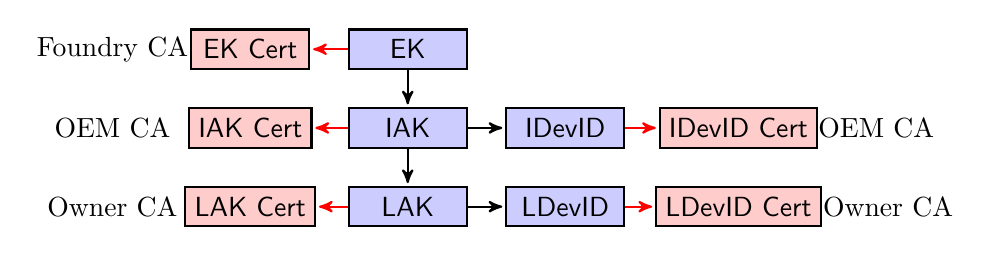
\begin{tikzpicture}[->,>=stealth',shorten >=1pt,auto,node distance=2.0cm,
  thick,key/.style={rectangle,fill=blue!20,draw,
    font=\sffamily,minimum height=5mm,minimum width=15mm},
  cert/.style={rectangle,fill=red!20,draw,
    font=\sffamily,minimum height=5mm,minimum width=15mm},
  label/.style={rectangle,font=\rmfamily,minimum height=5mm,minimum width=10mm}]

  \node[key] (EK) {EK};
  \node[key] (IAK) [node distance=1cm, below of=EK] {IAK};
  \node[key] (IDevID) [node distance=2cm, right of=IAK] {IDevID};
  \node[key] (LDevID) [node distance=1cm, below of=IDevID] {LDevID};
  \node[cert] (EKC) [node distance=2cm,left of=EK] {EK Cert};
  \node[cert] (IAKC) [node distance=2cm,left of=IAK] {IAK Cert};
  \node[cert] (IDevIDC) [node distance=2.2cm,right of=IDevID] {IDevID Cert};
  \node[key] (LAK) [node distance=1cm,below of=IAK] {LAK};
  \node[cert] (LAKC) [node distance=2cm,left of=LAK] {LAK Cert};
  \node[cert] (LDevIDC) [node distance=2.2cm,right of=LDevID] {LDevID Cert};
  \node[label] (ManCA) [node distance=1.75cm,left of=EKC]{Foundry CA};
  \node[label] (OEMCA1) [node distance=1.75cm,left of=IAKC]{OEM CA};
  \node[label] (OEMCA2) [node distance=1.75cm,right of=IDevIDC]{OEM CA};
  \node[label] (OwnerCA1) [node distance=1.75cm,left of=LAKC]{Owner CA};
  \node[label] (OwnerCA2) [node distance=1.9cm,right of=LDevIDC]{Owner CA};

  \path[every node/.style={font=\sffamily\small,fill=white,inner
    sep=1pt}]
  (EK) edge node[right=1mm] {} (IAK)
  (IAK) edge node[above=1mm] {} (IDevID)
  (IAK) edge node[right=1mm] {} (LAK)
  (LAK) edge node[above=1mm] {} (LDevID)
  ;

  \path[every node/.style={font=\sffamily\small,fill=white,inner
    sep=1pt}]
  (EK) edge [color=red] (EKC)
  (IAK) edge [color=red] (IAKC)
  (IDevID) edge [color=red] (IDevIDC)
  (LAK) edge [color=red] (LAKC)
  (LDevID) edge [color=red] (LDevIDC)
  ;

  
  % \path[every node/.style={font=\sffamily\small, fill=white,inner sep=1pt}]
  %   (NM) edge [bend left=30] node[above=1mm] {$\{(R,n,a)\}_{A^{-1}}$} (NME)
  %   (NME) edge [bend left=30] node[below=1mm] {$\{(E,n)\}_{T^{-1}}$} (NM)
  %   (IN) edge (NM)
  %   (NM) edge (OUT)
  %   ;
\end{tikzpicture}

%%% Local Variables: 
%%% mode: latex
%%% TeX-master: "nfm24.tex"
%%% End:

  \caption{Keys and certificates created by CA provisioning.
    Black arrows are trust relationships while red
    arrows denote key inclusion in certificates. Certificates are
    labeled with their associated CA~\citep{DevIDSpec-TCG}.}
  \label{fig:cert_rel}
\end{figure}

%%\subsection{Creating and Using DevIDs}
To reiterate, trust for creation of a new DevID is based on an existing 
certificate. Therefore, a chain of certificates can be used to verify 
a chain of trust to some trust anchor~\citep{DevIDSpec-TCG}.
%%Trust in new DevIDs is inherited from an existing chain back to a
%%trust anchor~\citep{DevIDSpec-TCG}. 
Since the IAK provides definitive evidence that a key belongs to a 
specific device, the IAK certificate serves as the trust anchor 
and is the root node in a chain of DevID certificates. Since an AK has 
the \verb|Restricted| attribute set, it has the ability to prove that 
some unknown key is loaded on the same TPM as itself.  AK certificates 
are thus used as the existing certificate in the provisioning of new DevIDs
and may be parent nodes in a chain of DevID certificates. 
All IDevID and LDevID certificates are leaf nodes.
The resulting structure showing relationships between the EK, DevIDs 
and certificates is shown in figure~\ref{fig:cert_rel}.

% \begin{enumerate}
% \item\label{ite:idTPM} Manufacturers produce TPMs provisioned with an
%   EK certificate binding the EK to a specific TPM. TPMs and EK
%   certificates are then distributed to Original Equipment
%   Manufacturers (OEMs) and represent roots-of-trust.
% \item\label{ite:idDevIni} OEMs produce devices with TPMs provisioned
%   with one or more IDevID certificates that bind an IDevID key to a
%   device. Devices are then distributed to end users (Owners).
% \item\label{ite:idDevLoc} Owners may optionally provision their TPMs
%   with one or more LDevID certificates that bind LDevID keys to their
%   device.
% \end{enumerate} 

% \noindent Modeling and verifying device identification provisioning
% using CAs in \ref{ite:idDevIni} and \ref{ite:idDevLoc} is the subject
% of this work.

% \begin{itemize}[itemsep=0pt,parsep=0pt,partopsep=0pt]
% \item \textsf{TPM Manufacturer}: Manufacturers produce TPMs provisioned with an
%   EK certificate binding the EK to a specific TPM.
%   \begin{itemize}[itemsep=0pt,parsep=0pt,partopsep=0pt]
%   \item The EK is initialized in an immutable, shielded location
%   \item The EK certificate is generated and signed by the TPM
%     Manufacturer's CA binding the EK to the TPM.
%   \end{itemize}
% \item \textsf{OEM}: OEMs produce devices with TPMs provisioned with
%   one or more Initial DevID (IDevID) certificates that bind an Initial
%   DevID (IDevID) key to a device.
%   \begin{itemize}[itemsep=0pt,parsep=0pt,partopsep=0pt]
%   \item \textsf{A}: The Initial AK (IAK) is created and verified by
%     the OEM's CA to have correct key properties and to be loaded on
%     the same TPM as the EK.
%   \item \textsf{B}: The Initial DevID (IDevID) is created and verified
%     by the OEM's CA to have the correct key properties and to be
%     loaded on the same TPM as the IAK.
%   \item \textsf{CA Signing}: The IAK certificate and IDevID
%     certificate are signed by the OEM's CA binding the IAK and IDevID
%     to this specific device.
%   \end{itemize}
% \item \textsf{Owner}: Owners may optionally provision their TPMs with
%   one or more Local DevIDs (LDevID) certificates binding Local DevID
%   (LDevID) keys to their specific device.
%   \begin{itemize}[itemsep=0pt,parsep=0pt,partopsep=0pt]
%   \item \textsf{C}: The LAK is created and verified by the Owner's CA
%     to have the correct key properties and to be loaded on the same
%     TPM as the IAK.
%   \item \textsf{D}: The LDevID is created and verified by the Owner's
%     CA to have the correct key properties and to be loaded on the same
%     TPM as the LAK.
%   \item \textsf{CA Signing}: The LAK certificate and LDevID
%     certificate are signed by the Owner's CA binding the LAK and
%     LDevID to this specific device.
%   \end{itemize}
% \end{itemize}



% \begin{figure}[htbp]
%   \begin{centering}
%   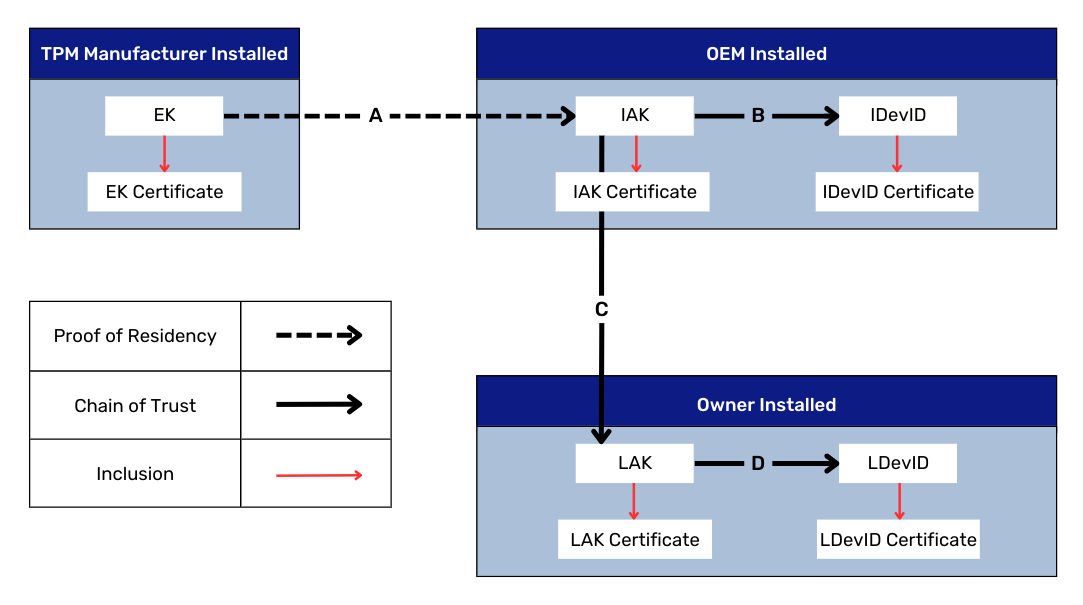
\includegraphics[width=\linewidth]{figures/certRelationships.png}
%   \par\end{centering}
%   \caption{Key and Certificate Relationships \citep{DevIDSpec-TCG}}
%   \label{fig:cert_rel}
% \end{figure}

\section{Protocol Execution Model}

TPM protocols are sequences of TPM Software Stack (TSS) instructions.  To model
protocol execution we use a labeled transition system representing
effects of protocol execution.  State is represented as a collection
of objects installed in the TPM while transitions perform operations
over state as defined by commands.  Labels represent individual
commands and label sequences represent protocols.  DevID provisioning
protocols are modeled as sequences of state transformations
corresponding with commands executed by the CA or certificate-requesting
entity.

%\subsection{Keys and Certificates}

The model defines a \verb|pubKey| and \verb|privKey| type for public
keys and private keys respectively. A key of either type requires a
unique identifier and a sequence of boolean values indicating the
presence of key attributes. An asymmetric key pair is a
\verb|pubKey| and a \verb|privKey| pair with the same identifier and
attributes.

% \begin{lstlisting}[language=Coq]
% Inductive pubKey : Type :=
% | Public : keyIdType -> Restricted -> Sign -> Decrypt -> FixedTPM -> pubKey.

% Inductive privKey : Type :=
% | Private : keyIdType -> Restricted -> Sign -> Decrypt -> FixedTPM -> privKey.
% \end{lstlisting}

Certificates are defined by the \verb|signedCert| type consisting of a
public key, an identifier, and a private key. The identifier
represents the certificate's Subject field and may include information
describing the TPM or the device. The private key parameter
denotes the CA's key that performed the signature over the
certificate.

% \begin{lstlisting}[language=Coq]
% Inductive identifier : Type :=
% | TPM_info : tpmInfoType -> identifier
% | Device_info : deviceInfoType -> identifier.

% Inductive signedCert : Type :=
% | Cert : pubKey -> identifier -> privKey -> signedCert.
% \end{lstlisting}

%\subsection{Commands}

Protocols used to create DevID certificates perform TPM, TSS and
non-TPM commands. A command may rely on a variety of parameters such
as keys, nonces, certificates, and messages that define structures an
entity may use or produce. The \verb|message| type shown in
Figure~\ref{fig:message-model} is an abstract representation of these
structures.

\begin{figure}[hbtp]
\vspace{-\medskipamount}
\vspace{-\medskipamount}

\begin{lstlisting}[language=Coq]
Inductive message : Type :=
| signature : message -> privKey -> message
| TPM2B_Attest : pubKey -> message
| encryptedCredential : message -> randType -> pubKey -> message
| TCG_CSR_IDevID : identifier -> signedCert -> pubKey -> message
| TCG_CSR_LDevID : message -> signedCert -> message 
| ...
\end{lstlisting}
\vspace{-\medskipamount}
\caption{TPM Message Model}
\label{fig:message-model}
\end{figure}

%% \begin{figure}[hbtp]
%% \begin{lstlisting}[language=Coq]
%%  Inductive message : Type :=
%%  | publicKey : pubKey -> message
%%  | privateKey : privKey -> message
%%  | hash : message -> message
%%  | signature : message -> privKey -> message
%%  | TPM2B_Attest : pubKey -> message
%%  | encryptedCredential : message -> randType -> pubKey -> message
%%  | randomNum : randType -> message
%%  | TCG_CSR_IDevID : identifier -> signedCert -> pubKey -> message
%%  | TCG_CSR_LDevID : message -> signedCert -> message
%%  | signedCertificate : signedCert -> message
%%  | pair : message -> message -> message.
%%  \end{lstlisting}
%%  \caption{TPM Message Model}
%%  \label{fig:message-model}
%%  \end{figure}

An entity may derive additional messages from a collection of known
messages.  For example, given a message of the form
\verb|signature m k|, \verb|m| may be deduced.  A message in the form
\verb|encryptedCredential n g k| protects its contents unless its
decryption key is also available.  Additional messages may be derived
from signed messages, \verb|TPM2B_Attest| structures, certificate
signing requests (CSRs), certificates, and message pairs. Other
messages contain no additional information or information is
concealed.  Message inference is modeled by a
recursive function \verb|inferFrom| and an equivalent inductive
proposition \verb|inferrable|.

\verb|tpm_state| and \verb|state| are lists of messages. The
\verb|tpm_state| type contains messages that a restricted signing key
may operate on. Such messages must be in one of two forms: (i) objects
constructed from TPM-internal data such as private keys and PCRs; or
(ii) digests produced by signature hash operations.  The \verb|state|
type contains messages visible to the system.

The labeled transition system models command execution in the
canonical fashion as a triple $(S,L,\rightarrow)$ where $S$ is a set
of states, $L$ is a set of labels, and
$\rightarrow \subseteq S \times L \times S$ is a labeled transition
relation.  In this case, $S$ is defined as \verb|tpm_state|$\times$\verb|state|
pairs; $L$ is the set of \verb|command| values; and $\rightarrow$ is
the \verb|execute| relation defining single command execution.
\verb|execute| is defined using an inductive proposition relating a
current state pair, a command, and a next state pair.

% \begin{figure}[h]
% \begin{lstlisting}[language=Coq]
% Inductive execute : tpm_state * state -> command -> tpm_state * state -> Prop
% \end{lstlisting}
% \caption{Type Signature of Execute Relation}
% \end{figure}

% Each \verb|command| constructor corresponds with one constructor in the
% \verb|execute| relation with the exception of \verb|TPM2_Sign| that
% corresponds with two. Each constructor possesses its own distinctive
% conditions that must be met for execution to succeed. These conditions
% are manifested in several ways: constructors pattern match on the
% command's inputs, some inputs must be in the current, and the results
% must be in the next state.

\begin{figure}[hbtp]
\vspace{-\medskipamount}
\vspace{-\medskipamount}
  \begin{footnotesize}
\begin{lstlisting}[language=Coq]
Inductive command : Type :=
| TPM2_Sign : message -> privKey -> command
| TPM2_Certify : pubKey -> privKey -> command
| TPM2_ActivateCredential : message -> privKey -> privKey -> command
| MakeCSR_IDevID : identifier -> signedCert -> pubKey -> command
| MakeCSR_LDevID : message -> signedCert -> command
| ...
\end{lstlisting}
\end{footnotesize}
\vspace{-\medskipamount}
\caption{TPM Command Data Structure}
\label{fig:command-model}
\end{figure}

%% \begin{figure}[hbtp]
%%  \begin{footnotesize}
%% \begin{lstlisting}[language=Coq]
%% Inductive command : Type :=
%% | TPM2_Hash : message -> command
%% | CheckHash : message -> message -> command
%% | TPM2_Sign : message -> privKey -> command
%% | TPM2_Certify : pubKey -> privKey -> command
%% | CheckSig : message -> pubKey -> command
%% | TPM2_MakeCredential : message -> randType -> pubKey -> command
%% | TPM2_ActivateCredential : message -> privKey -> privKey -> command
%% | MakeCSR_IDevID : identifier -> signedCert -> pubKey -> command
%% | MakeCSR_LDevID : message -> signedCert -> command
%% | CheckCert : signedCert -> pubKey -> command
%% | CheckAttributes : pubKey -> Restricted -> Sign -> Decrypt -> FixedTPM -> command
%% | MakePair : message -> message -> command.
%% \end{lstlisting}
%% \end{footnotesize}
%% \caption{TPM Command Data Structure}
%% \label{fig:command-model}
%% \end{figure}


% The \verb|TPM2_Hash| command performs a cryptographic hash operation
% on a piece of data. This data may be any message that is known to the
% entity performing the command \verb|state|. The result of the
% operation is abstractly defined using the opaque \verb|hash|
% constructor and is stored in both the next \verb|tpm_state| and
% \verb|state|.  The \verb|CheckHash| command verifies
% that the contents of a hash digest match a particular plaintext
% message. Both the hash digest and the plaintext message must be
% contained in the current \verb|state|.

% The \verb|TPM2_Sign| command generates a signature over a message
% using the specified private key.  To succeed the key must have the
% \verb|Sign| attribute set and the key must be present in
% \verb|tpm_state|. Execution then differs based on the status of the
% private key's \verb|Restricted| attribute. If the key does not have
% the \verb|Restricted| attribute set the message must simply be in
% \verb|state|. If the key does have the \verb|Restricted| attribute
% set, the message must be in the current \verb|tpm_state|.

While most TPM command behaviors are easily inferred from their name,
two are critical to CA protocol verification.  The \verb|TPM2_Certify|
command provides proof that an object is loaded in the TPM by
producing a signed \verb|TPM2B_Attest| structure. The command requires
two inputs: (i) a public key to be certified; and (ii) a private key
to sign the attestation structure. To execute, the TPM
verifies that the public key parameter's inverse is loaded.

% Messages produced by the \verb|TPM2_Sign| and \verb|TPM2_Certify|
% commands are defined using the \verb|signature| constructor. A
% signature may be verified against a public key using the
% \verb|CheckSig| command.

% The \verb|TPM2_MakeCredential| command is used when a remote entity,
% desires to affirm that some private key is loaded on the same TPM as a
% particular EK. This command produces an
% \verb|encryptedCredential| structure and requires three inputs: the
% cryptographic name of a key to be credentialed; a secret; and a public
% EK. % The cryptographic name of a key is produced by hashing its public
% % area with its associated hash algorithm and prepending the Algorithm
% % ID of the hashing algorithm.

The \verb|TPM2_ActivateCredential| command is used by the recipient of
an encrypted credential blob to release its secret.  The secret
contained in an encrypted credential blob is only released if the
credentialed key is loaded on the same TPM as the EK.  When executing
the \verb|TPM2_ActivateCredential| command, the TPM first decrypts the
blob with the EK then verifies that the private key corresponding with
the name field is also loaded. The secret is only released if both
steps succeed. The secret value may then be returned to the remote CA
to validate the result.

% The \verb|MakeCSR_IDevID| command produces a \verb|TCG_CSR_IDevID|
% structure.  A \verb|TCG_CSR_IDevID| is a certificate signing request
% (CSR) that contains the data required to couple an initial DevID to a
% TPM-containing device.  This structure is used any time
% a provisioning procedure uses the EK certificate.  The
% \verb|MakeCSR_LDevID| command is similar except that it produces a
% \verb|TCG_CSR_LDevID| structure that includes the certification
% information for a locally significant DevID.

% The \verb|CheckCert| command verifies a signature over a certificate
% against a public key. One should check an EK certificate against the
% public key of the TPM Manufacturer's CA, an IAK or IDevID certificate
% against the public key of the OEM's CA, and an LAK or LDevID
% certificate against the public key of the Owner's CA.  The
% \verb|CheckAttributes| command verifies a public key has all provided
% attributes.  In order to check the attributes, one must have have
% knowledge of that key. The key need not be loaded on a TPM since this
% command is typically used to check the attributes of some external
% entity's key.

%\subsection{Protocols}

Commands are sequenced linearly by the \verb|sequence| constructor to form
protocols. Protocol execution is defined as an inductive proposition
relating a current state pair, a command sequence, and a next state
pair. Sequential execution first executes the command at the head of a
sequence using the single command execution relation \verb|execute|
followed by executing the remaining sequence using the sequential
execution relation \verb|seq_execute|. The next state pair produced by
the single command becomes the current state pair for the following
sequence.

%% \begin{figure}[hbtp]
%% \begin{lstlisting}[language=Coq]
%% Inductive sequence : Type :=
%% | Sequence : command -> sequence -> sequence
%% | Done : sequence.
%% 
%% Inductive seq_execute : tpm_state * state -> sequence -> tpm_state * state -> Prop :=
%% | SE_Seq : forall ini mid fin c s,
%%     execute ini c mid ->
%%     seq_execute mid s fin ->
%%     seq_execute ini (Sequence c s) fin
%% | SE_Done : forall ini, seq_execute ini Done ini.
%% \end{lstlisting}
%% \caption{Sequential command execution model}
%% \label{fig:command-sequence-model}
%% \end{figure}

We prove an important property of sequential execution. That is,
sequential execution is deterministic. Given an initial state pair and
a command sequence, there is at most one final state pair that
satisfies the \verb|seq_execute| relation implying that command
sequence execution is a partial function. 
%% Second, sequential execution
%% is monotonic over state. Given a current state pair, command sequence,
%% and initial state pair, the initial state is always a subset of the
%% final state implying that command sequence execution is monotonic.

% \begin{figure}[hbtp]
%   \begin{lstlisting}[language=Coq]
%   Theorem seq_exec_deterministic : forall ini s fin1 fin2,
%     seq_execute ini s fin1 ->
%     seq_execute ini s fin2 ->
%     fin1 = fin2.
  
%   Theorem seq_exec_expansion : forall iniTPM ini s finTPM fin,
%     seq_execute (iniTPM,ini) s (finTPM,fin) ->
%     (iniTPM \subsetOf finTPM) /\ (ini \subsetOf fin).
%   \end{lstlisting}
%   \caption{Properties of Sequential Execution}
%   \label{fig:sequential-execution-properties}
%   \end{figure}

% For two commands to match, not only must the commands itself match but
% all of their inputs as well. To precisely describe this situation,
% this function utilizes the decidable equality property over the
% \verb|command| type. This requires declaring and proving that the
% \verb|command| type and all of the types it relies on (e.g.,
% \verb|message|, \verb|pubKey|, \verb|signedCert|) are members of the
% \verb|DecEq| class. These proofs may be conveniently automated.
%
%
%
\section{Proof Techniques}

The TCG describes several provisioning protocols~\citep{DevIDSpec-TCG}
that aim to maintain a cryptographic evidentiary chain linking a DevID
to a specific TPM and device. For each protocol, the specification
outlines steps for the CA and the certificate-requesting entity.  
%% The specification claims that each protocol provides certain assurances.
%% Each assurance manifests as an assertion regarding either
%% TPM-residency, key attributes, or previously-issued certificates and
%% provides the basis for the resulting cryptographic evidentiary chain
%% formed by a chain of certificates.
To verify the assurances provided by these protocols, 
we consider two scenarios: (i) the CA and certificate-requesting entity
perform the exact steps described by the specification; and (ii) only the 
CA is trusted to perform the steps described by the specification.
%% (i) the certificate-requesting entity 
%% and the CA are both trusted to execute
%% their steps correctly; and (ii) only the CA is trusted to execute its
%% steps correctly. 
We use two novel proof techniques to verify
TPM-residency --- \emph{minimal initial state} and
\emph{supersequence}.

\subsection{Minimal Initial State}

A minimal initial state aims to quantitatively describe the
prerequisites for executing a command sequence.  Given a command
sequence, a minimal initial state is defined as the smallest initial
state that allows successful execution of the sequence. The proof
obligation describing this property in
Figure~\ref{fig:minimal-initial-state} has two parts: (i) the minimal
initial state is a lower bound on the set of possible initial states;
and (ii) the minimal initial state is sufficient for successful
execution. 
\begin{figure}[hbtp]
\vspace{-\medskipamount}
\vspace{-\medskipamount}
\begin{lstlisting}[language=Coq]
Definition lower_bound seq minTPM min : Prop :=
  forall iniTPM ini fin,
  seq_execute (iniTPM, ini) seq fin ->
  (minTPM \subsetOf iniTPM) /\ (min \subsetOf ini).

Definition sufficient seq minTPM min : Prop :=
  exists fin, seq_execute (minTPM, min) seq fin.
\end{lstlisting}
\caption{Minimal Initial State}
\label{fig:minimal-initial-state}
\end{figure}
We use the minimal initial state in our verification of the first 
scenario to prove that an unknown key is
loaded on the same TPM as a previously-certified key when the
certificate-requesting entity follows the TCG's
recommended procedure.  
%% Specifically, the key whose presence is
%% required is included in the minimal initial state for protocol
%% execution.


\subsection{Supersequence}

A CA will only issue a certificate if it receives a valid \emph{certificate
signing request (CSR)}.  The production of a CSR shown in
Figure~\ref{fig:csr-production} can be described by these statements: 
the certificate-requesting
entity executes some arbitrary, unknown command sequence; the initial state
contains only messages that cannot be generated by the certificate-requesting 
entity itself; 
the command sequence produces some message in the final state; and a
CA determines that the message is a valid CSR.
We constrain the initial state of the certificate-requesting entity to
include only those that it cannot generate to ensure the contents of
the produced CSR are fresh. 

% A CA will only issue a certificate if it receives a valid
% certificate request. We model request validity by constraining the
% production of the request in the certificate-requesting entity.  The
% constraint is modeled as a set of restrictions on the useable elements
% of the entity's initial state. The \verb|needsGenerated| function
% defines the types of messages that must be generated by a command or
% command sequence. All messages except keys and certificates must be
% generated.

\begin{figure}[hbtp]
  \vspace{-\medskipamount}
  \vspace{-\medskipamount}
  \begin{lstlisting}[language=Coq]
Definition arbitrary_CSR_production (steps_CA : message -> Prop) : Prop :=
  forall seq iniTPM ini finTPM fin,
  seq_execute (iniTPM, ini) seq (finTPM, fin) ->
  (forall m', needsGenerated m' -> ~ In m' iniTPM) ->
  (forall m', needsGenerated m' -> ~ In m' ini) ->
  In csr fin ->
  steps_CA csr.
  \end{lstlisting}
  \caption{Arbitrary CSR production definition.}
  \label{fig:csr-production}
\end{figure}


%% In this case, the initial state may 
%% contain only keys and certificates.

To produce a valid CSR, specific commands
must be executed in a specific order.  Due to the shape of a valid
request and the checks performed by a CA, we can prove that any
command sequence that the certificate-requesting entity performed to
generate the request is a supersequence of the TCG-recommended procedure. 
A list is a supersequence of another list if and only if all the elements 
of the second list occur in order in the first --- the elements need not
occur consecutively. We use the supersequence techinque in our verification
of the second scenario to gain necessary knowledge of the unknown command
sequence executed by the certificate-requesting entity.
%% With this knowledge of the
%% certificate-requesting entity's behavior, we can apply an abbreviated
%% version of the minimal initial state technique to complete
%% verification.

\section{Identity Provisioning}

We consider two DevID provisioning protocols in detail: (i) Owner
creation of an LAK certificate based on an IAK certificate; and (ii)
OEM creation of an IAK certificate based on an EK certificate. For
each protocol, the TCG specification outlines steps for the CA and the
certificate-requesting entity. The specification claims that each
protocol provides certain assurances. Each assurance manifests as
an assertion regarding either TPM-residency, key attributes, or
previously-issued certificates and provides the basis for the
resulting cryptographic evidentiary chain formed by a chain of
certificates. We verify that each protocol guarantees its associated
assurances, thereby determining their correctness.

When verifying these goals, we consider two scenarios: (i) the
certificate-requesting entity and the CA are both trusted to execute
their steps correctly; and (ii) only the CA is trusted to execute its
steps correctly.  Because trust for a new certificate is rooted in an
existing certificate, these scenarios assume the precondition that
previously-issued certificates imply the assurances guaranteed by
their provisioning protocols.

\subsection{Owner Creation of LAK Certificate based on IAK Certificate}

The TCG's specification claims the protocol for creating an LAK
certificate in Figure~\ref{fig:lak-certificate-creation} provides
these assurances: (A) the LAK has good attributes; and (B) the LAK is
loaded on the same TPM as the IAK. These assurances correspond with
the Chain of Trust relation from IAK to LAK in Figure \ref{fig:cert_rel}.

\begin{figure}[hpbt]
  \vspace{-\medskipamount}
  \vspace{-\medskipamount}

  \begin{enumerate}[itemsep=0pt,parsep=0pt,partopsep=0pt]
  \setcounter{enumi}{-1}
  \item The Owner creates and loads the LAK
  \item The Owner certifies the LAK with the IAK
  \item The Owner builds the CSR% containing:
  % \begin{enumerate}[topsep=0pt, itemsep=0pt,parsep=0pt,partopsep=0pt]
  %   \item The signed \verb|TPM2B_Attest| structure
  %   \item The IAK certificate
  % \end{enumerate}
  \item The Owner takes a signature hash of the CSR
  \item The Owner signs the resulting hash digest with the LAK
  \item The Owner sends the CSR paired with the signed hash to the CA
  \item The CA verifies the received data% by checking:
  % \begin{enumerate}[topsep=0pt, itemsep=0pt,parsep=0pt,partopsep=0pt]
  %   \item The hash digest against the CSR
  %   \item The signature on the hash digest with the public LAK
  %   \item The signature on the \verb|TPM2B_Attest| structure with the public IAK
  %   \item The signature on the IAK certificate with the public key of the OEM's CA
  %   \item The attributes of the LAK
  % \end{enumerate}
  \item If all checks succeed, the CA issues the LAK certificate to the Owner
  \end{enumerate}
  \caption{LAK Certificate Creation Protocol}
  \label{fig:lak-certificate-creation}
\end{figure}

Modeling this protocol begins by initializing states for the Owner and
CA. The Owner must have its LAK, IAK, and IAK certificate, and the CA
must have its own key and the public key of the OEM's CA.  
% Private key values are represented by taking the inverse of the corresponding
% public key and are stored in the \verb|privLAK|, \verb|privIAK|, and
% \verb|privCA| variables. 
To enforce the randomness of cryptographic
keys, all key values are specified to be pairwise distinct.

% \begin{figure}[hbtp]
% \begin{lstlisting}[language=Coq]
% (* Owner parameters *)
% Parameter pubLAK : pubKey.
% Parameter pubIAK : pubKey.
% Parameter certIAK : signedCert.

% (* CA parameters *)
% Parameter pubCA : pubKey.
% Parameter pubOEM : pubKey.

% (* All keys are pairwise distinct *)
% Axiom keys_distinct :
%   pubLAK <> pubIAK /\
%   pubLAK <> pubCA /\
%   pubLAK <> pubOEM /\
%   pubIAK <> pubCA /\
%   pubIAK <> pubOEM /\
%   pubCA <> pubOEM.
% \end{lstlisting}
% \caption{Parameters of LAK Provisioning Procedure}
% \end{figure}

\begin{figure}[hpbt]
  \vspace{-\medskipamount}
  \vspace{-\medskipamount}
\begin{lstlisting}[language=Coq]
Definition steps1to5_Owner : sequence :=
TPM2_Certify pubLAK privIAK;
MakeCSR_LDevID (signature (TPM2B_Attest pubLAK) privIAK) certIAK;
TPM2_Hash (TCG_CSR_LDevID (signature (TPM2B_Attest pubLAK) privIAK) certIAK);
TPM2_Sign 
  (hash (TCG_CSR_LDevID (signature (TPM2B_Attest pubLAK) privIAK) certIAK))
  privLAK;
...
\end{lstlisting}
\caption{Owner's LAK Provisioning Protocol}
\label{fig:lak_model_Owner}
\end{figure}

The protocol is modeled in two parts: the Owner's steps (Steps 0-5)
followed by the CA's steps (Steps 6-7).  Each part of the procedure is
modeled using the initialized state and the sequential command
construction defined previously.  We construct a \verb|sequence| value
for the Owner and a function for the CA. Constructing the Owner's
steps is straightforward and shown in
Figure~\ref{fig:lak_model_Owner}. Step 0 is assumed to have been
performed previously since its results are already encapsulated in the
Owner's initialized state.  Each remaining step of the Owner
corresponds with exactly one command in the model, namely
\verb|TPM2_Certify| for Step 1, \verb|MakeCSR_LDevID| for Step 2,
\verb|TPM2_Hash| for Step 3, \verb|TPM2_Sign| for Step 4, and
\verb|MakePair| for Step 5.

The CA's steps in Figure~\ref{fig:lak_model_CA} are more complex as
they rely on the certificate signing request produced by the Owner. 
First, the CA waits to receive a request from the
Owner. The request must be in a specific
format to be considered valid. The CA then executes Step 6 of the
procedure defined by the sequence within \verb|seq_execute|. If
execution succeeds, the CA issues the LAK certificate to the Owner.
The model includes several additional parameters and criteria to serve
as a method for referencing elements of the certificate request
within proof statements.

\begin{figure}[hpbt]
\vspace{-\medskipamount}
\vspace{-\medskipamount}
\begin{lstlisting}[language=Coq]
Definition steps_CA (msg:message) (iak lak:pubKey) (cert:signedCert) : Prop :=
match msg with
| (pair (TCG_CSR_LDevID (signature (TPM2B_Attest k) k0') (Cert k0 id k_ca'))
        (signature m k')) =>
    iak = k0 /\ lak = k /\ cert = (Cert k0 id k_ca') /\
    seq_execute (iniTPM_CA, inferFrom msg ++ ini_CA)
      CheckHash m 
        (TCG_CSR_LDevID (signature (TPM2B_Attest k) k0') (Cert k0 id k_ca'));
      CheckSig (signature m k') k;
      CheckSig (signature (TPM2B_Attest k) k0') k0;
      CheckCert (Cert k0 id k_ca') pubOEM';
      CheckAttributes k Restricting Signing NonDecrypting FixedTPM;
    (iniTPM_CA, inferFrom msg ++ ini_CA)
| _ => False
end.
\end{lstlisting}
\caption{CA's LAK Provisioning Protocol}
\label{fig:lak_model_CA}
\end{figure}

Assurance A is proved under both scenarios simultaneously 
by using only the CA's function. 
The \verb|CheckAttributes| command in the CA's function corresponds with
Step 6 of the provisioning procedure.  It follows that successful
execution implies the LAK has all attributes required to be an
attestation key.

We now verify Assurance B under the conditions of the first scenario
where the Owner and the CA are both trusted to execute their steps
correctly. Recall that this proof trusts that the
previously-performed IAK provisioning guarantees its associated
assurances, specifically that the IAK has good attributes.

We construct a minimal initial state pair for \verb|steps1to5_Owner|
using the following intuition: (i) the private LAK and private IAK are
loaded on the same TPM because the LAK is certified by the IAK; and
(ii) the IAK certificate is known to the Owner because it is included
in the CSR.  The proof of the lower bound property uses this
intuition.  The proof of the sufficiency property uses the
constructors of the \verb|execute| relation to demonstrate that a next
state pair exists that satisfies the \verb|seq_execute| relation for
the minimal initial state pair and \verb|steps1to5_Owner|. This proof
relies on two conditions, the IAK has good attributes and that the CA
issues the LAK certificate.

% \begin{figure}[hbtp]
% \begin{lstlisting}[language=Coq]
% Definition minTPM_Owner : tpm_state := [ privateKey privLAK
%                                        ; privateKey privIAK ].

% Definition min_Owner : state := [ signedCertificate certIAK ].

% Lemma lower_bound_Owner : 
%   lower_bound steps1to5_Owner minTPM_Owner min_Owner.

% Lemma sufficient_Owner : forall msg,
%   attestationKey pubIAK ->
%   steps_CA msg pubIAK pubLAK certIAK ->
%   sufficient steps1to5_Owner minTPM_Owner min_Owner.
% \end{lstlisting}
% \caption{Minimal Initial State of Owner}
% \end{figure}

This analysis of the Owner's steps' prerequisites in the form of a
minimal initial state leads to the conclusion that the LAK and IAK
must be loaded on the same TPM for the Owner to execute its
steps. 
%This conclusion is manifest in the \verb|iniTPM_Owner| variable
% which contains both the private LAK and private IAK. 
Therefore, we have now confirmed that Assurance B is in fact guaranteed by the
protocol when we assume that both the Owner and the CA are trusted to
execute their steps correctly.


We now attempt verification of the same goal under the second scenario
where only the CA is trusted to execute its steps correctly. 
% We constrain the production of the certificate request and its contents
% to the Owner so that we can achieve the supersequence conclusion. 
We define a cascading collection of recursive functions to determine
whether a given command sequence is a supersequence of
\verb|steps1to5_Owner|.  Using the properties provided by the
\verb|arbitrary_CSR_production| definition, we prove the Owner's
arbitrary command sequence satisfies this function.
% This proof is
% troublesome if we make no assumptions about the Owner.  Because the
% certificate request and its contents must have been produced by some
% entity, we assume the Owner to be this entity.  Owner and its
% characteristics are represented as a series of assumptions: the Owner
% executes some unknown sequence of commands \verb|s|; \verb|s| produces
% a message \verb|msg| in the Owner's next \verb|state|; the Owner's
% initial \verb|tpm_state| only contains private keys; the Owner's
% initial \verb|state| only contains public keys and certificates; and
% the CA executes its procedure on the message \verb|msg|.

% \begin{figure}[hbtp]
% \begin{lstlisting}[language=Coq]
% Theorem lak_and_iak_in_TPM : forall s iniTPM ini finTPM fin msg iak lak cert,
%   seq_execute (iniTPM, ini) s (finTPM, fin) -> 
%   In msg fin ->
%   (forall m', needsGeneratedTPM m' -> ~ In m' iniTPM) ->
%   (forall m', needsGenerated m' -> ~ In m' ini) ->
%   steps_CA msg iak lak cert ->
%   In (privateKey (pubToPrivKey lak)) iniTPM
%   /\ In (privateKey (pubToPrivKey iak)) iniTPM
% \end{lstlisting}
% \caption{Next Verification Goal for LAK Provisioning Procedure}
% \label{fig:lak_goal}
% \end{figure}

% These assumptions do not impact the Owner's trustworthiness. The LAK,
% IAK, and IAK certificates are universally quantified making no
% reference to the Owner. The assumptions simply constrain the
% certificate request, \verb|msg|, and its contents to the Owner.  The
% restrictions on the Owner's initial state pair are the main
% contributors to this constraint. Due to the nature of command
% execution, the certificate request and its contents must have be
% produced by a command or contained in the initial state.  Therefore,
% restrictions placed on the initial state allow only those messages
% that cannot be generated by a command sequence.  The
% \verb|needsGeneratedTPM| function restricts the Owner's initial
% \verb|tpm_state| to include only previously created private keys while
% the \verb|needsGenerated| function restricts the Owner's initial
% \verb|state| to include public keys and previously issued
% certificates.  The subject of these certificates may be the Owner or
% another entity.  These restrictions prevent using other messages in the
% Owner state to build the certificate request.

% We cannot directly prove the new LAK is loaded on the same TPM as the
% IAK, but we can derive an important conclusion about the command
% sequence the Owner executes. Specifically, the sequence \verb|s| is a
% supersequence of the Owner's correct steps.  We define a cascading
% collection of recursive functions to determine whether a given command
% sequence is a supersequence of \verb|steps1to5_Owner|.  Using current
% assumptions about Owner and the CA we prove the Owner's unknown
% sequence \verb|s| satisfies this property. The proof relies on the
% structure of the certificate request as required by the CA's
% steps. To produce a message with this structure, specific
% commands must be executed in a specific order.

From here we need only demonstrate that the private LAK and private IAK
must be loaded on the same TPM to execute a command sequence with this property.
We do this by reusing the intuition described in the first scenario that
the private LAK and private IAK are loaded on the same TPM if the LAK
is certified by the IAK.
% Next we demonstrate the Owner must have executed \verb|TPM2_Certify|
% on the public LAK and private IAK.  Recall our conclusion that the LAK
% and IAK must be loaded on the same TPM if the LAK is certified using
% the IAK. Using the previous conclusion it is trivial to prove this
% command is contained within the Owner's sequence \verb|s|.  We use the
% function \verb|command_in_sequence| to describe this scenario.  We
% prove one last set of intermediate lemmas that show that the LAK and
% IAK must be loaded on the same TPM to execute any sequence that
% contains this command.  The composition of these small proofs leads to
% the goal shown in Figure \ref{fig:lak_goal}. 

Due to extra parameters and criteria of the \verb|steps_CA| function,
the formal theorem states that the inverse of the key contained in the
IAK certificate and the inverse of the key contained in the new
certificate are loaded on the same TPM. This is the assertion made by
Assurance B.  Therefore, we have proven that Assurance B is guaranteed
by the protocol assuming only the CA is trusted to execute its steps
correctly.

The procedure uses the previously provisioned IAK to prove the new LAK
is loaded on the same TPM and thus contained in the device identified
by the IAK certificate. Thus, when issuing the LAK certificate, the CA
should use the same device identifying information as the IAK
certificate's Subject field. To summarize, Assurance A is guaranteed
by the attribute check performed by the CA and Assurance B is
guaranteed by the IAK's \verb|Restricted| attribute and the signed
\verb|TPM2B_Attest| structure.

\subsection{OEM Creation of IAK Certificate based on EK Certificate}

The TCG's specification claims the procedure in
Figure~\ref{fig:iak-creation} guarantees three assurances: (A) the IAK
has good attributes; (B) the IAK is loaded on the same TPM as the EK;
and (C) the EK certificate is valid. These assurances correspond with
the Proof of Residency line A in Figure \ref{fig:cert_rel}.

\begin{figure}[hbtp]
\vspace{-\medskipamount}
\vspace{-\medskipamount}
\begin{enumerate}[itemsep=0pt,parsep=0pt,partopsep=0pt]
  \setcounter{enumi}{-1}
  \item The OEM creates and loads the IAK
  \item The OEM builds the CSR% containing:
  % \begin{enumerate}[topsep=0pt, itemsep=0pt,parsep=0pt,partopsep=0pt]
  %   \item Device identity information including the device model and serial
  %   number
  %   \item The EK certificate
  %   \item The IAK public area
  % \end{enumerate}
  \item The OEM takes a signature hash of the CSR
  \item The OEM signs the resulting hash digest with the IAK
  \item The OEM sends the CSR paired with the signed hash to the CA
  \item The CA verifies the received data% by checking:
  % \begin{enumerate}[topsep=0pt, itemsep=0pt,parsep=0pt,partopsep=0pt]
  %   \item The hash digest against the CSR
  %   \item The signature on the hash digest with the IAK public key
  %   \item The signature on the EK certificate with the public key of the TPM Manufacturer's CA
  %   \item The attributes of the IAK
  % \end{enumerate}
  \item If all of the checks succeed, the CA issues a challenge blob to the OEM% by:
  % \begin{enumerate}[topsep=0pt, itemsep=0pt,parsep=0pt,partopsep=0pt]
  %   \item Calculating the cryptographic name of the IAK
  %   \item Generating a nonce
  %   \item Building the encrypted credential structure
  % \end{enumerate}
  \item The OEM releases the secret nonce by decrypting the challenge
    blob and verifying the IAK name
  \item The CA checks the returned nonce against the one generated in Step 6b
  \item If the check succeeds, the CA issues the IAK certificate to the OEM
  \end{enumerate}
  \caption{IAK Certificate Creation Protocol}
  \label{fig:iak-creation}
\end{figure}

% Modeling this protocol begins by defining parameters for the OEM and
% CA. The OEM has its IAK, EK, EK certificate, and device identifying
% information and the CA has its own key, the public key of the TPM
% Manufacturer's CA, and a secret nonce.

% \begin{figure}[hbtp]
% \begin{lstlisting}[language=Coq]
% (* OEM parameters *)
% Parameter pubIAK : pubKey.
% Parameter pubEK : pubKey.
% Parameter certEK : signedCert.
% Parameter devInfo : deviceInfoType.

% (* CA parameters *)
% Parameter pubCA : pubKey.
% Parameter pubTM : pubKey.
% Parameter nonce : randType.
% \end{lstlisting}
% \caption{Parameters of IAK Provisioning Procedure}
% \end{figure}

The procedure from Figure~\ref{fig:iak-creation} is similar to the one
described in Figure~\ref{fig:lak-certificate-creation}. 
% All steps except for step 1 and
% part of step 6 are included. 
We focus on the details that differ from
the previous verification process.

The provisioning procedure may be viewed as the composition of four
parts: the OEM's initial steps (Steps 0-4) followed by the CA's
initial steps (Steps 5-6) followed by the OEM's final step (Step 7)
followed by the CA's final steps (Steps 8-9). The initial steps of the
OEM and the OEM's CA are constructed similarly to the steps of the
Owner and the Owner's CA respectively.  The OEM's final step is
naturally constructed as a simple function. First the OEM waits to
receive a challenge blob from the CA, then the OEM executes Step
7. The CA's final steps are implicit in the proof statements and do
not require an explicit definition.

Proving Assurance A is trivial and proceeds identically to the
corresponding proof in the previous section. Proving Assurance C is
also quite similar since the CA checks the signature on the EK
certificate with the public key of the TPM Manufacturer's CA. 
% The command
% \verb|CheckCert (Cert k0 id0 k_ca') pubTM| in the CA's function
% corresponds with Step 5 of the provisioning procedure. The CA's
% function binds the EK to the variable \verb|k0| and the EK certificate
% to the message \verb|Cert k0 id0 k_ca'|.  Successful execution of this
% command directly implies that EK certificate is valid.

%% Figure is not referenced in the paper, thus pulling it to get back
%% a page
% \begin{figure}[hbtp]
% \begin{lstlisting}[language=Coq]
% Definition steps_CA (msg : message) (ident : identifier) (ek iak : pubKey) (cert : signedCert) : Prop :=
%   match msg with
%   | (pair (TCG_CSR_IDevID (Device_info id) (Cert k0 id0 k_ca') k) (signature m k')) =>
%         ident = (Device_info id) /\ ek = k0 /\ iak = k /\ cert = (Cert k0 id0 k_ca') /\
%         seq_execute   (iniTPM_CA, inferFrom msg ++ ini_CA)
%                       (CheckHash 
%                           msg 
%                          (TCG_CSR_IDevID (Device_info id) (Cert k0 id0 k_ca') k) ;;
%                        CheckSig 
%                          (signature m k') 
%                           k ;;
%                        CheckCert 
%                          (Cert k0 id0 k_ca') 
%                           pubTM ;;
%                        CheckAttributes 
%                           k 
%                           Restricting Signing NonDecrypting Fixing ;;
%                        TPM2_Hash 
%                          (publicKey k);;
%                        TPM2_MakeCredential 
%                          (hash (publicKey k))
%                           nonce
%                           k0 ;;
%                        Done)
%                       (hash (publicKey k) ::iniTPM_CA, 
%                        encryptedCredential (hash (publicKey k)) nonce k0 :: hash (publicKey k) 
%                        ::inferFrom msg ++ ini_CA)
%   | _ => False
%   end.

% Definition step7_OEM (msg : message) : sequence :=
% TPM2_ActivateCredential 
%     msg 
%     privEK 
%     privIAK ;;
% Done.
% \end{lstlisting}
% \caption{Partial Model of IAK Provisioning Procedure}
% \label{fig:iak_model}
% \end{figure}

We now verify Assurance B when the OEM and the CA are both trusted to
execute their steps correctly. We implement the same strategy as
before showing that the private IAK and private EK are contained in
the OEM's minimal initial \verb|tpm_state|. We build a minimal initial
state pair for the composition of \verb|steps1to4_OEM| and
\verb|step7_OEM| using the following intuition: (i) the EK certificate
and public IAK are known to the Owner because they are included in the
CSR; and (ii) the private IAK and private EK are loaded on the same TPM
because the IAK is credentialed by the EK. The two required proofs to
determine minimality proceed similarly to the corresponding proof in
the previous section.

We now attempt to verify the same goal assuming only the CA is trusted
to execute its steps correctly. 
We modify the \verb|arbitrary_CSR_production| definition 
so that we can describe the additional interaction
that takes place between the OEM and the CA. We now say that
the OEM executes some arbitrary sequence of commands \verb|seq1|;
\verb|seq1| produces some message \verb|csr| in the OEM's intermediate
state; the OEM's initial state contains only messages that need not be
generated; the CA executes its steps on \verb|csr| and sends the
challenge blob \verb|encryptedCredential (hash (publicKey iak)) g ek|
to the OEM; the OEM executes some other arbitrary command sequence \verb|seq2|;
and \verb|seq2| releases the secret nonce value \verb|g| into the OEM's
final state. The CA's final steps are implicit in that the nonce in
the challenge blob is the same nonce in the OEM's state.

\begin{figure}[hptb]
\vspace{-\medskipamount}
\vspace{-\medskipamount}
\begin{lstlisting}[language=Coq]
Theorem iak_and_ek_in_TPM :
  forall seq2 seq1 iniTPM ini midTPM mid finTPM fin csr ident ek iak cert g,
  seq_execute (iniTPM, ini) seq1 (midTPM, mid) -> 
  In csr mid ->
  (forall m', needsGeneratedTPM m' -> ~ In m' iniTPM) ->
  (forall m', needsGenerated m' -> ~ In m' ini) ->
  steps_CA csr ident ek iak cert ->
  seq_execute
   (midTPM, inferFrom (encryptedCredential (hash (publicKey iak)) g ek)++mid)
    seq2 
   (finTPM, fin) ->
  In (randomNum g) fin ->
  In (privateKey (pubToPrivKey iak)) iniTPM /\ 
  In (privateKey (pubToPrivKey ek)) iniTPM.
\end{lstlisting}
\caption{Final Verification Goal for IAK Provisioning Procedure}
\label{fig:iak_goal}
\end{figure}

From here we prove that \verb|seq2| is a supersequence of the OEM's
correct final steps (i.e., Step 7). This proof uses two important
properties of sequential execution. The first being that one cannot
produce a random number in its final state without an encrypted
credential containing that number in its initial state. The second
being the converse of the first, one cannot produce an encrypted
credential containing a particular random number in its final state
without that number or an encrypted credential containing that number
in its initial state.

We reuse the intuition from the first scenario to show that the private
IAK and private EK are loaded on the same TPM if the IAK is
credentialed by the EK.
% Our next step is to demonstrate that the OEM must in fact have
% executed \verb|TPM2_ActivateCredential| on the challenge blob using
% the private EK and private IAK. This result is a direct consequence of
% the supersequence conclusion. We then verify that execution of a
% sequence containing this command implies that the EK and IAK are
% loaded on the same TPM.  
The composition of these intermediate proofs leads
to our goal shown in Figure~\ref{fig:iak_goal}.  Due to the extra
parameters and criteria of the \verb|steps_CA| function, the proof
statement shows that the inverse of the key contained in the EK
certificate and the inverse of the key contained in the new
certificate are loaded on the same TPM. This is precisely the
assertion described by Assurance B.

In conclusion, we use the previously-certified EK to prove that the new
IAK is loaded on the same TPM as itself. When issuing the IAK
certificate, the CA uses the device identifying information from the
recieved CSR.  Assurance A is guaranteed by the attribute check
performed by the CA, Assurance B is guaranteed by the EK's
\verb|Restricted| attribute and the secret contained in the challenge
blob, and Assurance C is guaranteed by the signature check on the EK
certificate performed by the CA.

Our analysis revealed a potential inconsistency in how the IAK
provisioning procedure is described. The procedure provides no
assurance regarding IAK device-residency as implied by its definition.
The IAK certificate is intended to provide evidence that a key belongs
to a specific device, yet the procedure makes no guarantees that the
IAK is actually on the device.  Proving an IAK belongs to a specific
device requires first binding the IAK to a specific TPM using the EK
and then binding the TPM to a specific device \citep{DevIDSpec-TCG}.
However, the CA makes no attempt at performing the second part of this
process. Instead the CA fully trusts the OEM to have provided the
correct device identifying information.

Even the attestation variation of the IAK provisioning procedure does
not attempt verification. This variation uses a quote over selected
PCRs to show only that the device is running the appropriate, trusted
firmware. All devices with the same model number have an identical
golden hash value that represents its expected PCR digest.  Although
this check guarantees that the TPM containing the IAK is on a specific
\textit{type} of device it does not guarantee that the TPM is on a
specific \emph{device}.

A small change to the attestation variation of IAK provisioning
procedure will overcome this shortcoming. The TPM should store a
measurement that contains a device's unique identifier. In this way,
each individual device has a unique golden hash value and its identity
can be uniquely determined.  Due to integrity guarantees of the TPM's
PCR mechanism, this modification provides definitive evidence that a
key belongs to a specific device. A weakness of this modification
is it requires a large database of golden hash values. Maintaining
such a database in dynamic environments with many devices would be
challenging.  however, the approach will be useful in critical systems
where it is imperative to know the precise identity of a specific
device.
%
%
%
\section{Related Work}
The Privacy CA protocol for the TPM 1.2 has been extensively studied
using various formal methods.  The work
of~\citet{PrivacyCAAnalysis-Chen} analyzes the Privacy CA protocol in
the presence of an adversary. They suggest a small modification to the
protocol that enhances its security without changing the existing
functionality of the TPM 1.2. Our work similarly suggests a small
modification to the IAK provisioning procedure which requires no
change to the existing functionality of the TPM 2.0.  In contrast,
earlier work of~\citet{PrivacyCAAnalysis-Hall} analyzes the Privacy CA
protocol but does not consider any specific adversary. Instead, they
consider the functional correctness of the protocol and specifically
examine the protocol implementation to ensure that it produces correct
results.  Our current work has many parallels to earlier
work~\citep{PrivacyCAAnalysis-Hall} where we verified TPM 1.2 CA
protocols.  Specifically, modeling TPM command execution as a
transition system over an abstract system state using a monadic
approach. Here we implement a state transition system directly over a
smaller subset of TPM 2.0 commands and non-TPM commands targeted to
device identifiers.

The TPM 1.2 Privacy CA protocol was replaced by the Direct Anonymous
Attestation (DAA) scheme in the TPM 2.0.  The work
of~\citet{DAAAnalysis-Whit} and~\citet{DAAAnalysis-Wes} thoroughly
study the TPM 2.0 DAA scheme.  Collectively, they develop a symbolic
model, a C++ implementation, and a formally-verified fix of the
scheme. Both the Privacy CA and DAA protocols aim to allow remote
authentication of a device while maintaining its anonymity. As such
these protocols differ from the key certification protocols analyzed
here that provide individual device identification.

Other work uses formal techniques to examine various aspects of both
the TPM 1.2~\citep{AuthAnalysis,PCRAnalysis} and
2.0~\citep{EAAnalysis,HMACAnalysis}.  These include analyzing
authentication~\citep{AuthAnalysis}, platform configuration registers
(PCRs)~\citep{PCRAnalysis}, enhanced authorization
(EA)~\citep{EAAnalysis}, and hash-based message authentication code
(HMAC) mechanisms~\citep{HMACAnalysis}. They utilize tools and
techniques such as SAPIC~\citep{kremer2016automated},
Tamarin~\citep{meier2013tamarin}, and stateful applied pi
calculus~\citep{Milner:99:Communicating-a}, amongst others.
% 
%
%
\section{Conclusions and Future Work}

Contributions of this research include: (i) design and implementation
of an abstract formal model of TPM command execution; (ii) an in-depth
analysis of the TCG-provided IAK and LAK certification protocols;
and (iii) a recommendation for clarifying the IAK provisioning
procedure.  To perform this verification we used two primary proof
techniques.  The first uses a minimal initial state to ensure key
residency while the second uses a command supersequence to characterize
arbitrary construction of a certificate request.

This work is motivated by the need for strong identifiers in
performing layered remote
attestation~\cite{Coker::Principles-of-R,Ramsdell:2019aa,helble2021flexible}.
It is essential that an attestation result be strongly bound to the
attestation manager that produced it. LAKs are ideal for identifying
attestation managers and providing a secure method for signing
attestation results.  Verification results reported here allow safe
integration of LAKs into our verified attestation tool
suite~\cite{petz2022innovations}.

Improvements are necessary should we choose to extend our approach to
a broader range of DevID protocols.  An initial step would expand the
command library to include additional TPM and TSS commands necessary
for modeling the attestation variation of both provisioning
protocols. The attestation variations use PCRs to inform a remote CA
of a certificate-requesting entity's state. This variation is strongly
encouraged during to ensure the CA it is issuing a certificate to a
device running trusted software. To include necessary PCR-related
commands, the structure of abstract state should be modified from a
pair to a record similar to that of the work of
\citet{PrivacyCAAnalysis-Hall}.

\medskip

\noindent All verification models and \LaTeX\ source associated with
this work may be found at \url{git@github.com:ku-sldg/nfm24.git}.

% 
% 
% ---- Bibliography ----
%
% BibTeX users should specify bibliography style 'splncs04'.
% References will then be sorted and formatted in the correct style.
%
%\bibliographystyle{splncs04}
\bibliographystyle{splncsnat}
%\bibliography{sldg}
\bibliography{bib/sldg,bib/thesis_bibliography}
%
\end{document}
